\documentclass[a4paper, oneside, onecolumn, 11pt]{memoir}
\newenvironment{code}{\captionsetup{type=listing}}{}

%\begin{code}
%    \caption{Den skrevne Pythonkode.
%    \label{kode}}

%    \inputminted[firstline=20, lastline=30,
%        frame=single, framesep=2mm, fontsize=\footnotesize, linenos% Spanning over more than one page!
%    ]{python}{kode.py}
%\end{code}

% Preamble
\usepackage{preamble}

\graphicspath{{./Graphics/}}

\title{Logbook}
\author{Anne Kirstine Knudsen\thanks{anne839i97@gmail.com} \and Laurits N. Stokholm\thanks{laurits.stokholm@post.au.dk}}
\date{\today}

\begin{document}
\maketitle
%\tableofcontents

\section{Problem and Aim}
% What is the problem
\begin{itemize}
    \item Set up a Michelson Interferometer
    \item Determination of the expansion coefficient of a piezoelectric element
    \item Study the effect of intensity differences of the interferometer arms
\end{itemize}


\subsection{Research method}
\begin{figure}[h!]
    \centering
    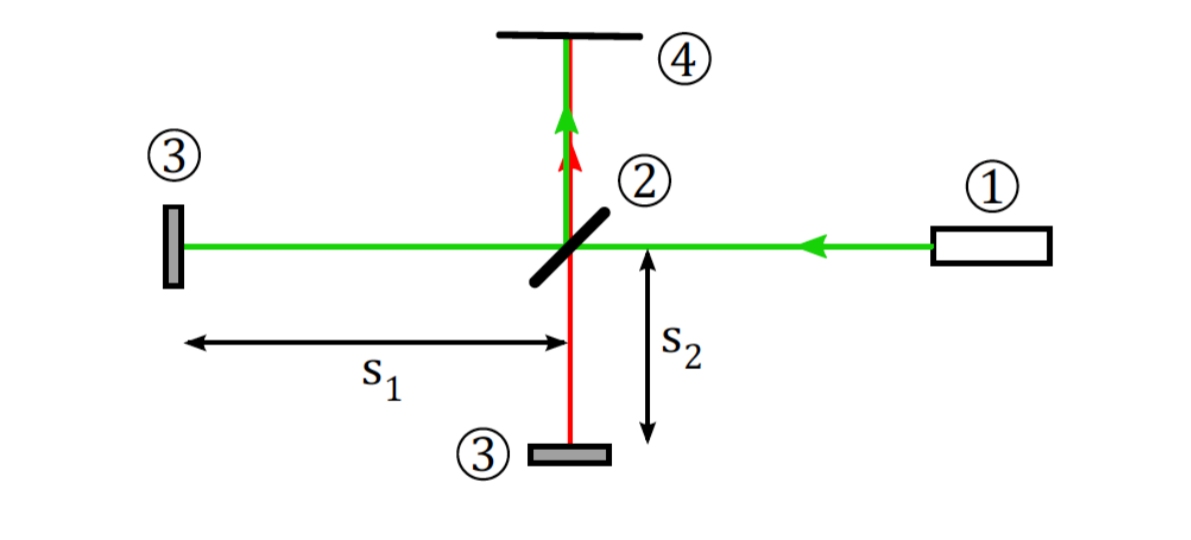
\includegraphics[width=\columnwidth]{michelsonsetup}
        \caption{Sketch of a Michelson interferometer. The beam from the laser (1) is aimed at the beam splitter (2) which divides the beam into two partial beams. The two beams are reflected by the mirrors (3). An interference pattern can be observed on the screen/detector (4)}
    \label{fig:michelsonsetup}
\end{figure}

\subsubsection{Planning}
% Start each entry by stating what you are planning to do


\subsubsection{Experimental Equipment Available}
% What is the experimental 
\begin{minipage}[h]{0.5\textwidth}
    \flushleft{%
    \begin{itemize}
        \item Breadboard
        \item HeNe-laser
        \item Photo-detector
        \item 4 mirrors
        \item 1 Pieze element
        \item 3 Lenses $(f= \SI{50}{\mm}, \SI{-50}{\mm}, \SI{150}{\mm})$
    \end{itemize}
}
\end{minipage}
\begin{minipage}[h]{0.5\textwidth}
    \flushright{%
    \begin{itemize}
        \item 2 beam splitter cubes
        \item 1 $\frac{\lambda}{4}$-plate
        \item 1 Neutral density filter wheel
        \item A glass cell
        \item 2 Black dumping screens
        \item Set of screwdrivers + powersupplies
    \end{itemize}
}
\end{minipage}

\subsubsection{Practical/ Technical notes}
One should be aware of the following:

 \renewcommand{\labelenumi}{\Roman{enumi}}
\begin{enumerate}
    \item The optical breadboard with all its components is very heavy, so take care when taking it out of the cabinet and back again.
    \item Remember laser light can be harmful, so be careful also with parasitical beams!
    \item Remember not to touch any optics on the surfaces on which light in impinging!  
    \item Do only apply voltages in the range 0-10V to the control input of the piezodriver,
        and do not drive it at a frequency of more than 200 Hz. Hence, check and 
        adjust the output of the function generator with the Pico Scope before  
        connecting it to the piezo-driver. The voltage delivered to the piezo should be a   
        factor of 10 higher than the control voltage (check backside of the piezo-driver).
    \item Remember to take clear pictures of you various setups, including the 
        electronic wiring. 
    \item At the end of each experimental session, remember to safely fix all the optical 
        elements to the breadboard in positions similar to those on Fig. 1., and bring   
        everything back in good order in the cabinets!

\end{enumerate}

\subsubsection{Critical issues}
% What are the critical issues?

\subsubsection{Strategy}
% How to carry out the tasks
% Strategy for carry out the experiments
% - which parameter have to be meassured and how to best do it
% - taking reflections into account

\subsection{Setup}
% Make a sketch of the experiment, explain why this setup.

\subsection{Laboratory setup}
% Does it work as expected
% Did you chose to go differently than originally sketched?
% Add pictures

%\subsection{Raw data}
%% Screen shots and link to data files
%
%% 1st Meassurement
%%slit width 2, 0.5 mm
%
%\subsection{Fast analysis}
%% Does the data seem to be valid?
%% Do you see any sign of systematic errors?
%
%\subsection{Conclusion}
%% What have you learned?
%% What has or could be done differently for improving the results?
%Her og der og alle vegne, som du kan se på \cref{SourceCode:1}
%
%\begin{code}
%	\caption{Caption
%    \label{SourceCode:1}}
%    \inputminted[firstline=1, lastline=5, frame=single, framesep=2mm, fontsize=\footnotesize, linenos% Spanning over more than one page!
%]{python}{kode.py}
%\end{code}

\end{document}

